\documentclass[14pt,aspectratio=169]{beamer}
\usetheme{Marburg}
\graphicspath{{Arquivos/}}
\usepackage[utf8]{inputenc}
\usepackage[english]{babel}
\usepackage[T1]{fontenc}
\usepackage{amsmath}
\usepackage{amsfonts}
\usepackage{amssymb}
\usepackage{graphicx}
\author{R. Zhang ,N. Kabadi , P. Punnen }
\newcommand{\TT}{The minimum spanning tree problem with conflict constraints and its variations}
\newcommand{\TB}{Texte Biblique}
\newcommand{\DT}{}
\newcommand{\IN}{ Introduction}
\newcommand{\PI}{I - Cas de résolution polynomiale et infaisabilité}
\newcommand{\PII}{II - Formule de programmation entiére et borne inf}
\newcommand{\PIII}{III - Borne supérieure et heuristique}
\newcommand{\PIV}{IV - Test d'infaisabilité}
\newcommand{\PV}{V - résultats}
\newcommand{\CO}{Conclusion}
\newcommand{\Qst}{Questions}

\title{\TT}
%\setbeamercovered{transparent} 
\setbeamertemplate{navigation symbols}{\href{https://github.com/katiamedjani}{https://github.com/katiamedjani}} 
\logo{
\includegraphics[scale=0.033]{LogoReformada}} 
%\institute{Igreja Presbiteriana Central} 
\date{19 Avril 2019} 
%\subject{} 
\begin{document}

\begin{frame}
\titlepage
\end{frame}

%\LARGE

\begin{frame}
 \tableofcontents
\end{frame}

\section{\IN}
\begin{frame}{\IN}{\TT}
 \begin{table}
  \begin{center}
  
    \begin{itemize}
        \item MST est polynomial
        \item MSTC est NP-hard
        \item graphe Cactus, le probléme de faisabilité est limité polynomialement, alors que la version d'optimalité reste NP-Hard.
        \item d'autre cas où MSTC peut être résolut en temps polynomial.
    \end{itemize}   
  
  \end{center}
 \end{table}
\end{frame}



\section{\PI}
\begin{frame}{\PI}{\TT}\pause
 \textbf{Graph cactus} \newline
 \begin{figure}[H!]
     \centering
     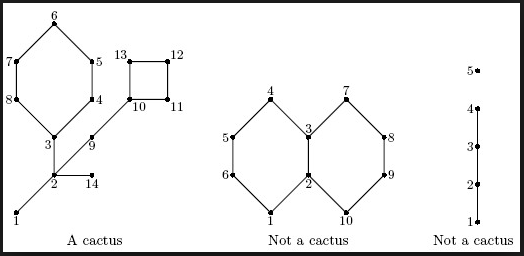
\includegraphics[width=0.4\textwidth]{cactus1.png}
     \caption{Cactus Graph}
     \label{fig:my_label}
 \end{figure}
 \pause
 Quand un graphe est un Cactus le probléme de faisabilité peut être résolu en temps polynomial.\pause \newline Tandis que le probléme d'optimalité reste NP-hard.
\end{frame}

\begin{frame}{\PI}{\TT}
 soit G=(V,E), \pause
 S ensemble des conflit, choisit arbitrairement.
 $(E_{1}, E_{2}, ..., E_{k})$ une partition de E.
 \newline $E_{i}={e_{1,i}, e_{2,i},..., e_{l_{i},i}}$ l'ensemble des arêtes du cycle i.
\end{frame}

\begin{frame}{\PI}{\TT}
 \begin{block}{Infaisabilité du problème MSTC pour les graphes cactus}
 $\exists$ plus d'un ensemble de type $\{e_{p,i}, e_{q,i}\} \in S$.
 \newline Si l'intersection de des ensembles est vide donc pas de solution.
 \newline Sinon $e_{p,i} \in$ X.
 \end{block}
\end{frame}

\begin{frame}{\PI}{\TT}
\begin{block}{Théorème 1}
 MSTC problem on a cactus is NP-hard. However, its feasibility version can be solved in $ O ( max \{| E |, | S |\})$ time.
%We say that the conflict set (conflict relation) S is transitive if and only if for distinct e, f, g in E, \{e, f\} \in S, nad \{f, g\} \in S, imply \{ e, g\} \in S.
 \end{block}
 \begin{block}{G2SAT}
 On demontre que le problème MSTC est équivalent au problème 2-SAT pondéré. 
 \newline
 A partir du résultat de 2-SAT pondéré, la version de faisabilité du MSTC cactus est résoluble en temps (max \{|E|,|S|\}). Tandis que l'optimalité reste NP-hard
 \end{block}
\end{frame}


\begin{frame}{\PI}{\TT}
 \begin{block}{Lemme 2}
The conflict graph Ĝ is a collection of disjoint cliques if and only if the conflict set S is transitive.
 \end{block}
 
 on démontre que MSTC peut être résolu en temps polynomial si Ĝ est transitif.
\end{frame}

\begin{frame}{\PI}{\TT}
 \begin{block}{Lemme 3}
 When the conflict graph is a collection of disjoint cliques (equivalently when S is transitive), MSTC can be solved in polynomial time.
 \end{block}
\end{frame}

\begin{frame}{\PI}{\TT}
 \begin{block}{Théorème 4}
Suppose the conflict graph Ĝ is such that deletion of a fixed number, k, of nodes, that can be identified in polynomial time, reduces Ĝ to a collection of node-disjoint cliques. Then the corresponding instance of MSTC can be solved in polynomial time.
 \end{block}
 \begin{itemize}
     \item Preuve
 \end{itemize}

\end{frame}

\begin{frame}{\PI}{\TT}
 \begin{block}{Corrolaire 5}
SIf the conflict graph has a fixed number k of edges, which can be identified in polynomial time, so that deletion of these edges makes the conflict graph a collection of disjoint cliques, then MSTC can be solved in polynomial time.
 \end{block}
\end{frame}

 \begin{frame}{\PI}{\TT}
 \begin{block}{Lemme 6}
If $ M \subseteq E $ is a maximum cardinality matching in G and OPT is the optimum objective function value of Max-ECP on G then $|M| \geqslant \frac{OPT}{\delta}$.
 \end{block}
 \begin{itemize}
     \item Preuve
 \end{itemize}
\end{frame}

 \begin{frame}{\PI}{\TT}
 \begin{block}{Max-ECP}
Le probléme est de trouver une partition de V en ensembles disjoints $V_{1}, V_{2},...V_{m}$ tel que $\forall$ 1$\leq$i $\leq$m, chaque deux arêtes de $V_{i}$ sont adjacentes et le nombre total d'arêtes de $V_{1}, V_{2},...V_{m}$ est maxmimum.
 \end{block}
\end{frame}

 \begin{frame}{\PI}{\TT}
 \begin{block}{Théorème 07}
If Approx-Clique(G) computes an $\epsilon$-optimal solution to the maximum clique problem on G, then the approximate greedy algorithm computes a ( 3$\epsilon $- 1 ) optimal solution to Max-ECP on G. Further if the complexity of Approx-Clique(G) is $O ( f ( m , n ))$ then the complexity of the approximate greedy algorithm is O(nf( m , n )) .
 \end{block}
 \begin{itemize}
     \item Preuve
 \end{itemize}
\end{frame}

%\section{\PIV}
%\begin{frame}{\PIV}{\TT}

%\end{frame}

%\section{\PV}
%\begin{frame}{\PV}{\TT}

%\end{frame}

%\section{\CO}
%\begin{frame}{\CO}{\TT}

%\end{frame}


\end{document}